%\section{Experiment and Analysis}
%\label{sec:experiment}
%% Clean the words connect the model to the results
%
%In this section, we introduce our in-field measurement experiments, 
%and analyze the resulting impact on various network parameters.

% Subsec Experiment design
\section{In-field Experimentation}
\label{subsec:measurements}

In this section, we introduce our in-field measurement experiments, 
and analyze the results.
In-field measurements are very useful in understanding real world environmental and temporal channel effects. 


\subsection{Spectral Wardriving}
\label{subsec:spectrummeasurements}
When it comes to heterogeneous networks that can be configured over numerous channels with different spectral activity, such information is vital in determining an optimal network configuration. 
To this end, we collected spectral user activity measurements in several typical areas including metropolitan, campus, and suburban locations in Dallas, TX, as seen in Fig.~\ref{fig:measurement_map}. 
They were gathered over 24 hours on weekdays in distinct areas to offer insight into differing channel types. 
From these measurements, we extract channel state variation over time, location information, and user mobility patterns present in each area.

\begin{figure}
\vspace{-0.0in}
\centering
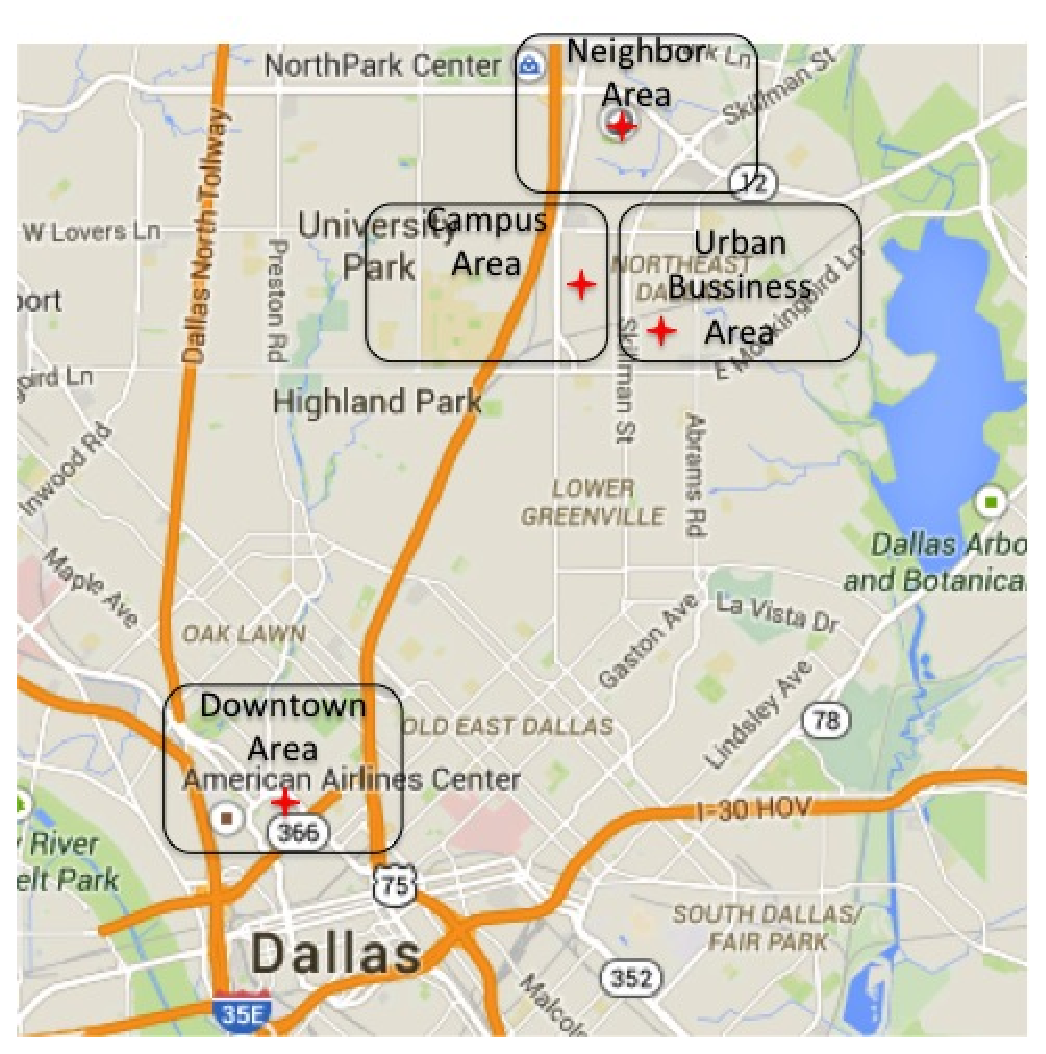
\includegraphics[width=84mm]{figures/measurements_map}
\vspace{-0.1in}
\caption{Long Term Measurements Locations}
\label{fig:measurement_map}
\vspace{-0.3in}
\end{figure}

In each of the location, we left our equipment running to collect channel state information measurements for 24 hours during weekdays. 
% Experiment equipment
For hardware, we employ a Rohde \& Schwarz FSH8 portable spectrum that operates in frequencies from 100 KHz to 8 GHz. 
This portable spectrum analyzer is controlled by a Python script on a laptop that records the received signal strength over time.
% Data normalize 
To the best of our knowledge, there is no commercial readily available, mobile, multiband antenna from 450 MHz to 5.2 GHz on the market. 
Due to this limitation, we use a 700-MHz mobile antenna to perform in-field measurements and normalize the mobile antenna gain across all bands with indoor experimentation. 
To do so, we use a Universal Software Radio Peripheral (USRP) N210 to generate signals at 450 MHz, 800 MHz, and 2.4 GHz. 
We feed these signals directly to the spectrum analyzer and adjust the configuration of USRP to make the received signal strength the same as the 5.2 GHz signal from Gateworks 2358 with a XR5 radio. 
We then connect the signal source to a fixed multiband antenna (QT 400 Quad Ridge Horn Antenna) and measure the received signal at a fixed distance with the 700 MHz antenna and antennas for different bands to obtain the antenna loss for each band. 
We adjust the received signal strength collected via the 700-MHz mobile antenna according to this normalization.
We use $-85 dBm$ as a threshold in the activity level calculation for the normalized data.

% Introduce how to calculate the achieved capacity
% Explain multiband and activity level
When wireless devices operate in WiFi bands, the channel separation is relatively small (e.g., 5 MHz for the 2.4 GHz band). 
As a result, many works assume that the propagation characteristics across different channels are similar. 
However, with the large frequency differences between WiFi and white space bands (e.g., multiple GHz), propagation becomes a key factor in the deployment of wireless networks with both bands.
Here, a frequency band is defined as a group of channels which have little frequency separation, meaning they have similar propagation characteristics.
In this work, we consider the diverse propagation and activity characteristics for four total frequency bands: 450 MHz, 800 MHz, 2.4 GHz, and 5.2 GHz.
We refer to the two former frequency bands as white space bands and the two latter frequency bands as WiFi bands.
The differences in propagation and spectrum utilization create opportunities for the joint use of white space and WiFi bands in wireless access networks according to the environmental characteristics (e.g., urban or rural and downtown or residential) of the deployment location.


Through the measured data set, we are able to calculate the activity level via Eq.~\ref{eq:actdef}.
We calculate a single activity level over a one minute time window, followed by averaging these activity levels every 30 minutes across the 24 hour data set duration.

\begin{table*}
\centering % centering table 
\begin{tabular}{|l|c|c|c|c|c|c|c|c|c|c|c|c|c|} % creating 13 columns 
\hline %\hline % inserting double-line 
%Bands     & \multicolumn{3}{c|}{Dallas} & \multicolumn{3}{c|}{Weatherford} & \multicolumn{3}{c|}{Millsap} \\% [0.5ex]
%\hline % inserts single-line 
% Entering 1st row 
%Area Type & Downtown & Residential & Suburban & Downtown &  Residential & Sparse & Downtown & Residential & Sparse \\ % [0.5ex]
%\hline % inserts single-line 
%\multirow{8}{*}{Downtown}	
%&\multirow{2}{*}{Downtown 450 MHz}	
%&0:00-11:00 &  22.09 &  21.27 &  22.28 &  22.47 &  21.65 &  21.68&  22.37 &  22.16&  23.12 &  22.73&  22.01 &  22.54 \\ 	
%\cline{3-15}	
%&&12:00-23:00&  21.80 &  20.86 &  21.80 &  22.54 &  22.35 &  22.61&  22.45 &  21.58&  22.18 &  23.09&  22.11 &  22.09 \\ 	
%\cline{2-15}	
%&\multirow{2}{*}{800 MHz}	
%&0:00-11:00 &  12.99 &  12.44 &  12.08 &  12.32 &  11.60 &  11.60&  12.48 &  12.10&  11.14 &  11.55&  11.98 &  11.12 \\ 	
%\cline{3-15}	
%&&12:00-23:00&  11.88 &  12.27 &  12.36 &  12.05 &  12.15 &  14.00&  13.32 &  12.29&  11.38 &  11.55&  12.92 &  13.16 \\ 	
%\cline{2-15}	
%&\multirow{2}{*}{2.4 GHz}	
%&0:00-11:00 &  29.08 &  29.15 &  29.49 &  28.93 &  29.01 &  28.86&  28.84 &  29.53&  29.03 &  28.74&  34.89 &  29.15 \\ 	
%\cline{3-15}	
%&&12:00-23:00&  28.60 &  29.61 &  29.44 &  28.55 &  28.05 &  28.62&  28.74 &  28.93&  28.26 &  27.73&  28.19 &  29.85 \\ 	
%\cline{2-15}	
%&\multirow{2}{*}{5.2 GHz}	
%&0:00-11:00 &  27.21 &  27.11 &  26.20 &  25.77 &  26.70 &  26.17&  25.67 &  26.10&  25.77 &  25.41&  26.05 &  26.34 \\ 	
%\cline{3-15}	
%&&12:00-23:00&  26.17 &  26.03 &  25.19 &  26.41 &  26.80 &  25.17&  26.08 &  25.60&  26.44 &  26.58&  25.50 &  25.45 \\ 	
%\hline	
%\multirow{8}{*}{Urban}	
%&\multirow{2}{*}{450 MHz}	
%&0:00-11:00 &  23.17 &  23.69 &  23.45 &  22.83 &  23.24 &  23.43&  23.48 &  23.74&  23.69 &  23.36&  23.29 &  23.00 \\ 	
%\cline{3-15}	
%&&12:00-23:00&  22.85 &  22.81 &  23.62 &  23.74 &  23.14 &  23.48&  23.38 &  22.52&  22.04 &  22.59&  22.59 &  22.42 \\ 	
%\cline{2-15}	
%&\multirow{2}{*}{800 MHz}	
%&0:00-11:00 &  12.63 &  13.20 &  13.08 &  12.94 &  11.55 &  11.48&  11.60 &  11.38&  11.86 &  11.72&  10.47 &  10.32 \\ 	
%\cline{3-15}	
%&&12:00-23:00&  12.00 &  11.86 &  10.71 &  11.93 &  12.72 &  12.36&  11.48 &  11.43&  11.72 &  11.60&  11.72 &  11.91 \\ 	
%\cline{2-15}	
%&\multirow{2}{*}{2.4 GHz}	
%&0:00-11:00 &  29.04 &  28.66 &  27.29 &  28.15 &  27.89 &  27.72&  28.18 &  27.38&  28.18 &  27.74&  28.15 &  27.96 \\ 	
%\cline{3-15}	
%&&12:00-23:00&  27.96 &  29.14 &  28.97 &  28.20 &  28.80 &  29.57&  29.02 &  27.72&  27.70 &  27.77&  29.21 &  28.42 \\ 	
%\cline{2-15}	
%&\multirow{2}{*}{5.2 GHz}	
%&0:00-11:00 &  25.41 &  25.29 &  26.32 &  26.49 &  27.23 &  27.28&  26.99 &  26.27&  25.36 &  26.13&  25.81 &  24.88 \\ 	
%\cline{3-15}	
%&&12:00-23:00&  26.92 &  26.49 &  26.41 &  27.11 &  25.67 &  26.53&  26.73 &  26.97&  26.32 &  25.79&  27.57 &  26.65 \\ 	
%\hline	
%\multirow{8}{*}{Campus}	
%&\multirow{2}{*}{Campus 450 MHz}	
%&0:00-11:00 &  20.29 &  21.56 &  21.41 &  22.52 &  23.12 &  21.97&  21.65 &  21.63&  21.87 &  21.22&  21.17 &  21.39 \\ 	
%\cline{3-15}	
%&&12:00-23:00&  22.33 &  22.88 &  22.28 &  21.65 &  22.49 &  22.16&  21.32 &  22.35&  21.56 &  21.75&  21.75 &  20.45 \\ 	
%\cline{2-15}	
%&\multirow{2}{*}{800 MHz}	
%&0:00-11:00 &  11.98 &  12.20 &  12.68 &  12.03 &  11.52 &  11.19&  11.96 &  12.94&  11.52 &  11.93&  12.44 &  10.95 \\ 	
%\cline{3-15}	
%&&12:00-23:00&  11.26 &  11.62 &  12.12 &  12.70 &  12.34 &  11.62&  11.57 &  12.17&  11.55 &  12.08&  11.88 &  11.98 \\ 	
%\cline{2-15}	
%&\multirow{2}{*}{2.4 GHz}	
%&0:00-11:00 &  26.10 &  25.91 &  28.02 &  26.61 &  27.90 &  27.09&  27.01 &  27.21&  26.99 &  26.75&  25.69 &  26.46 \\ 	
%\cline{3-15}	
%&&12:00-23:00&  26.58 &  27.23 &  26.92 &  26.29 &  26.10 &  26.13&  26.25 &  25.53&  25.79 &  25.84&  26.13 &  26.46 \\ 	
%\cline{2-15}	
%&\multirow{2}{*}{5.2 GHz}	
%&0:00-11:00 &  26.68 &  26.05 &  25.12 &  25.93 &  25.36 &  25.79&  26.03 &  26.73&  25.89 &  25.26&  25.81 &  25.50 \\ 	
%\cline{3-15}	
%&&12:00-23:00&  25.19 &  25.60 &  24.52 &  25.00 &  26.08 &  26.17&  26.85 &  26.53&  26.10 &  25.53&  25.89 &  25.31 \\ 	
%\hline	
%\multirow{8}{*}{Neighborhoods}	
%&\multirow{2}{*}{450 MHz}	
%&0:00-11:00 &  23.17 &  24.35 &  23.82 &  23.75 &  23.44 &  22.76&  24.08 &  25.26&  24.54 &  23.87&  23.82 &  23.70 \\ 	
%\cline{3-15}	
%&&12:00-23:00&  23.48 &  22.67 &  23.53 &  23.48 &  23.99 &  24.49&  23.99 &  22.98&  22.86 &  23.03&  23.89 &  23.63 \\ 	
%\cline{2-15}	
%&\multirow{2}{*}{Neighborhoods 800 MHz}	
%&0:00-11:00 &  15.72 &  16.30 &  16.33 &  15.72 &  16.54 &  14.48&  14.62 &  14.48&  15.68 &  15.03&  15.60 &  16.33 \\ 	
%\cline{3-15}	
%&&12:00-23:00&  15.72 &  14.74 &  14.74 &  14.38 &  15.41 &  15.00&  15.84 &  16.25&  14.84 &  14.69&  15.51 &  14.93 \\ 	
%\cline{2-15}	
%&\multirow{2}{*}{2.4 GHz}	
%&0:00-11:00 &  26.49 &  26.37 &  26.22 &  26.03 &  24.97 &  27.16&  27.76 &  26.56&  26.05 &  26.22&  25.74 &  27.18 \\ 	
%\cline{3-15}	
%&&12:00-23:00&  27.01 &  26.34 &  25.79 &  25.48 &  26.53 &  26.29&  25.33 &  25.86&  26.92 &  25.98&  25.48 &  27.66 \\ 	
%\cline{2-15}	
%&\multirow{2}{*}{5.2 GHz}	
%&0:00-11:00 &  25.93 &  26.27 &  25.07 &  25.67 &  26.77 &  26.80&  27.52 &  25.38&  25.55 &  25.86&  25.62 &  26.13 \\ 	
%\cline{3-15}	
%&&12:00-23:00&  25.29 &  26.49 &  26.70 &  26.77 &  25.31 &  24.59&  24.78 &  25.91&  25.67 &  24.73&  24.73 &  25.21 \\ 	

%Subtable here
&& \multicolumn{12}{c|}{Activity Level (Percentage)}  \\
\hline
\multirow{2}{*}{Downtown 450 MHz}	
&0:00-11:00 &  22.09 &  21.27 &  22.28 &  22.47 &  21.65 &  21.68&  22.37 &  22.16&  23.12 &  22.73&  22.01 &  22.54 \\ 	
\cline{2-14}	
&12:00-23:00&  21.80 &  20.86 &  21.80 &  22.54 &  22.35 &  22.61&  22.45 &  21.58&  22.18 &  23.09&  22.11 &  22.09 \\ 	
\hline
\multirow{2}{*}{Campus 450 MHz}	
&0:00-11:00 &  20.29 &  21.56 &  21.41 &  22.52 &  23.12 &  21.97&  21.65 &  21.63&  21.87 &  21.22&  21.17 &  21.39 \\ 	
\cline{2-14}	
&12:00-23:00&  22.33 &  22.88 &  22.28 &  21.65 &  22.49 &  22.16&  21.32 &  22.35&  21.56 &  21.75&  21.75 &  20.45 \\ 	
\hline
\multirow{2}{*}{Neighborhoods 800 MHz}	
&0:00-11:00 &  15.72 &  16.30 &  16.33 &  15.72 &  16.54 &  14.48&  14.62 &  14.48&  15.68 &  15.03&  15.60 &  16.33 \\ 	
\cline{2-14}	
&12:00-23:00&  15.72 &  14.74 &  14.74 &  14.38 &  15.41 &  15.00&  15.84 &  16.25&  14.84 &  14.69&  15.51 &  14.93 \\ 	
\hline	
\end{tabular}    
\caption{Part of Activity Level in Multiple Locations} % title name of the table 
\label{tab:activitymeasurement}    
\vspace{-0.4in}
\end{table*}    


% Data analysis
% List part of the data
Due to the limited space, the full list of measurements are available upon request, but part of the measurement results are listed in Table~\ref{tab:activitymeasurement}.
Through these activity level results, we can see several interesting differences between bands and locations.
The activity levels on the 450 MHz band have almost the same patterns across each of the four measured areas. 
The large propagation area of the relatively low 450 MHz frequency can influence the areas simultaneously and the patterns seen play out regularly on weekdays.
The suburban neighborhood area has more activity in 800 MHz than other types of areas, but the 800 MHz activity levels are relatively low compared to the other bands in all areas.
The WiFi 2.4 GHz channel in suburban neighborhoods has more activity in the night while the downtown area has more activity in the day time.
The campus has more WiFi activities in the morning than the afternoon and night. 
We integrate these activity level results into our numerical simulation using our GSR algorithm later in this section.


\subsection{Crowdsourcing User Mobility}
\label{subsec:mob_measurements}
% Mobility pattern measurements
To identify user mobility patterns, we leverage the data from WiEye application database to analyze user locations across time.
% WiEye introduction
The WiEye application created for the data collection is currently available for download and usage via the Google Android Market. 
Our application offers connection quality information for WiFi access points in both graphical and tabular form as a download incentive. 
All data collected is done so as a background process, either continuously while the user is running the application or periodically if the user has opted in to background data collection for SMU research. 
Additionally, the data collected has been approved by the Southern Methodist University Institutional Review Board, a human subjects research committee, ensuring that all ethical precautions have been taken in collecting user data with our application.


% Wieye cluster
User mobility data has a direct impact on the power consumption and resource allocation of a wireless network.
% other cities range Here, discuss the wieye data process, 
For our user mobility analysis, we pull data from the WiEye database in several Texas cities, including Houston, Dallas, San Antonio, and Austin in weekdays from October 1st 2014 to March 20th 2015.
For accuracy concerns, we removed all data points with reported speeds above $30km/h$.
We first query the all Dallas measurements in the range restricted latitudinally from 
$32.7471 S$ to $33.2153 S$, and longitudinally from $97.1677 W$ to $96.5600 W$.
We then superimpose the same area from Dallas over Houston, Austin, San Antonio according to the difference of latitude and longitude between the center of the cities as defined by Google maps.
We split each area into 36 grid districts as shown in Fig~\ref{fig:wieye_map}, quantize time into six 4-hour slots per day, and record in each grid the number of unique users according to the device ID records from the WiEye database.
We compress the data set into one weekday since WiEye reports the measurements with an uncertain gap and the data set has a limited number of users.


\begin{figure}[h]
\vspace{-0.0in}
\centering
\includegraphics[width=74mm]{figures/wieye_cluster_map}
\vspace{-0.1in}
\caption{WiEye District Grids}
\label{fig:wieye_map}
\vspace{-0.1in}
\end{figure}

%\begin{table*}[hpt]	
\begin{minipage}{.5\linewidth}	
\centering	
\begin{tabular}{|c|c|p{0.4cm}|p{0.4cm}|p{0.4cm}|p{0.4cm}|p{0.4cm}|p{0.4cm}|p{0.4cm}|}	
\hline	
Period & Total User &\multicolumn{7}{c|}{User Distribution in 36 Grid} \\	
\hline	
&& & 1 &2 & 3 & 4 & 5&6\\	
\cline{3-9}	
 & \multirow{7}{*}{145}	
 &A	
& 0& 0& 0& 0& 0& 0  \\	
\cline{3-9}	
 && B	
& 0& 0& 12& 20& 2& 0  \\	
\cline{3-9}	
0:00 && C	
& 0& 7& 44& 30& 0& 0  \\	
\cline{3-9}	
 -&& D 	
& 0& 0& 0& 22& 0& 0  \\	
\cline{3-9}	
4:00 && E 	
& 0& 8& 0& 0& 0& 0  \\	
\cline{3-9}	
 && F 	
& 0& 0& 0& 0& 0& 0  \\	
\hline	
\end{tabular}	
\vspace*{0.1in} \\	
\begin{tabular}{|c|c|p{0.4cm}|p{0.4cm}|p{0.4cm}|p{0.4cm}|p{0.4cm}|p{0.4cm}|p{0.4cm}|}	
\hline	
Period & Total User &\multicolumn{7}{c|}{User Distribution in 36 Grid} \\	
\hline	
&& & 1 &2 & 3 & 4 & 5&6\\	
\cline{3-9}	
 & \multirow{7}{*}{152}	
 &A	
& 0& 0& 0& 0& 0& 0  \\	
\cline{3-9}	
 && B	
& 0& 3& 6& 19& 0& 0  \\	
\cline{3-9}	
4:00 && C	
& 0& 31& 35& 27& 0& 0  \\	
\cline{3-9}	
 -&& D 	
& 0& 0& 0& 28& 0& 0  \\	
\cline{3-9}	
8:00 && E 	
& 0& 3& 0& 0& 0& 0  \\	
\cline{3-9}	
 && F 	
& 0& 0& 0& 0& 0& 0  \\	
\hline	
\end{tabular}	
\vspace*{0.1in} \\	
\begin{tabular}{|c|c|p{0.4cm}|p{0.4cm}|p{0.4cm}|p{0.4cm}|p{0.4cm}|p{0.4cm}|p{0.4cm}|}	
\hline	
Period & Total User &\multicolumn{7}{c|}{User Distribution in 36 Grid} \\	
\hline	
&& & 1 &2 & 3 & 4 & 5&6\\	
\cline{3-9}	
 & \multirow{7}{*}{217}	
 &A	
& 0& 4& 0& 4& 0& 0  \\	
\cline{3-9}	
 && B	
& 0& 19& 7& 11& 0& 4  \\	
\cline{3-9}	
8:00 && C	
& 0& 56& 51& 24& 2& 0  \\	
\cline{3-9}	
 -&& D 	
& 0& 3& 0& 18& 4& 0  \\	
\cline{3-9}	
12:00 && E 	
& 0& 10& 0& 0& 0& 0  \\	
\cline{3-9}	
 && F 	
& 0& 0& 0& 0& 0& 0  \\	
\hline	
\end{tabular}	
\vspace*{0.1in} \\	
\end{minipage}	
\begin{minipage}{.5\linewidth}	
\centering	
\begin{tabular}{|c|c|p{0.4cm}|p{0.4cm}|p{0.4cm}|p{0.4cm}|p{0.4cm}|p{0.4cm}|p{0.4cm}|}	
\hline	
Period & Total User &\multicolumn{7}{c|}{User Distribution in 36 Grid} \\	
\hline	
&& & 1 &2 & 3 & 4 & 5&6\\	
\cline{3-9}	
 & \multirow{7}{*}{267}	
 &A	
& 0& 0& 0& 0& 0& 0  \\	
\cline{3-9}	
 && B	
& 0& 7& 14& 28& 2& 4  \\	
\cline{3-9}	
12:00 && C	
& 0& 58& 64& 18& 0& 0  \\	
\cline{3-9}	
 -&& D 	
& 0& 2& 12& 30& 7& 0  \\	
\cline{3-9}	
16:00 && E 	
& 0& 14& 2& 2& 0& 0  \\	
\cline{3-9}	
 && F 	
& 0& 0& 3& 0& 0& 0  \\	
\hline	
\end{tabular}	
\vspace*{0.1in} \\	
\begin{tabular}{|c|c|p{0.4cm}|p{0.4cm}|p{0.4cm}|p{0.4cm}|p{0.4cm}|p{0.4cm}|p{0.4cm}|}	
\hline	
Period & Total User &\multicolumn{7}{c|}{User Distribution in 36 Grid} \\	
\hline	
&& & 1 &2 & 3 & 4 & 5&6\\	
\cline{3-9}	
 & \multirow{7}{*}{292}	
 &A	
& 0& 3& 0& 0& 0& 0  \\	
\cline{3-9}	
 && B	
& 0& 18& 10& 22& 0& 4  \\	
\cline{3-9}	
16:00 && C	
& 0& 76& 75& 27& 0& 3  \\	
\cline{3-9}	
 -&& D 	
& 0& 0& 7& 34& 7& 0  \\	
\cline{3-9}	
20:00 && E 	
& 0& 6& 0& 0& 0& 0  \\	
\cline{3-9}	
 && F 	
& 0& 0& 0& 0& 0& 0  \\	
\hline	
\end{tabular}	
\vspace*{0.1in} \\	
\begin{tabular}{|c|c|p{0.4cm}|p{0.4cm}|p{0.4cm}|p{0.4cm}|p{0.4cm}|p{0.4cm}|p{0.4cm}|}	
\hline	
Period & Total User &\multicolumn{7}{c|}{User Distribution in 36 Grid} \\	
\hline	
&& & 1 &2 & 3 & 4 & 5&6\\	
\cline{3-9}	
 & \multirow{7}{*}{190}	
 &A	
& 0& 0& 0& 3& 0& 0  \\	
\cline{3-9}	
 && B	
& 0& 2& 16& 14& 2& 3  \\	
\cline{3-9}	
20:00 && C	
& 0& 32& 54& 23& 0& 0  \\	
\cline{3-9}	
 -&& D 	
& 0& 7& 3& 23& 0& 0  \\	
\cline{3-9}	
24:00 && E 	
& 0& 8& 0& 0& 0& 0  \\	
\cline{3-9}	
 && F 	
& 0& 0& 0& 0& 0& 0  \\	
\hline	
\end{tabular}	
\vspace*{0.1in} \\	
\end{minipage}	
\label{table:austin_cluster}	
\caption{User Distribution in Districts of Austin}	
\end{table*}	

%\begin{table*}[hpt]	
\begin{minipage}{.5\linewidth}	
\centering	
\begin{tabular}{|c|c|p{0.4cm}|p{0.4cm}|p{0.4cm}|p{0.4cm}|p{0.4cm}|p{0.4cm}|p{0.4cm}|}	
\hline	
Period & Total User &\multicolumn{7}{c|}{User Distribution in 36 Grid} \\	
\hline	
&& & 1 &2 & 3 & 4 & 5&6\\	
\cline{3-9}	
 & \multirow{7}{*}{288}	
 &A	
& 0& 11& 14& 8& 0& 0  \\	
\cline{3-9}	
 && B	
& 0& 16& 12& 8& 6& 12  \\	
\cline{3-9}	
0:00 && C	
& 0& 11& 28& 32& 6& 3  \\	
\cline{3-9}	
 -&& D 	
& 0& 2& 24& 12& 22& 4  \\	
\cline{3-9}	
4:00 && E 	
& 0& 20& 6& 8& 2& 0  \\	
\cline{3-9}	
 && F 	
& 0& 8& 3& 10& 0& 0  \\	
\hline	
\end{tabular}	
\vspace*{0.1in} \\	
\begin{tabular}{|c|c|p{0.4cm}|p{0.4cm}|p{0.4cm}|p{0.4cm}|p{0.4cm}|p{0.4cm}|p{0.4cm}|}	
\hline	
Period & Total User &\multicolumn{7}{c|}{User Distribution in 36 Grid} \\	
\hline	
&& & 1 &2 & 3 & 4 & 5&6\\	
\cline{3-9}	
 & \multirow{7}{*}{237}	
 &A	
& 0& 8& 7& 8& 0& 0  \\	
\cline{3-9}	
 && B	
& 0& 20& 7& 4& 12& 7  \\	
\cline{3-9}	
4:00 && C	
& 0& 12& 12& 24& 4& 0  \\	
\cline{3-9}	
 -&& D 	
& 0& 0& 19& 11& 22& 0  \\	
\cline{3-9}	
8:00 && E 	
& 0& 20& 7& 2& 4& 0  \\	
\cline{3-9}	
 && F 	
& 0& 7& 8& 12& 0& 0  \\	
\hline	
\end{tabular}	
\vspace*{0.1in} \\	
\begin{tabular}{|c|c|p{0.4cm}|p{0.4cm}|p{0.4cm}|p{0.4cm}|p{0.4cm}|p{0.4cm}|p{0.4cm}|}	
\hline	
Period & Total User &\multicolumn{7}{c|}{User Distribution in 36 Grid} \\	
\hline	
&& & 1 &2 & 3 & 4 & 5&6\\	
\cline{3-9}	
 & \multirow{7}{*}{460}	
 &A	
& 0& 4& 26& 6& 8& 4  \\	
\cline{3-9}	
 && B	
& 0& 24& 15& 23& 28& 7  \\	
\cline{3-9}	
8:00 && C	
& 0& 38& 44& 30& 12& 4  \\	
\cline{3-9}	
 -&& D 	
& 0& 12& 30& 11& 30& 4  \\	
\cline{3-9}	
12:00 && E 	
& 0& 6& 28& 14& 2& 4  \\	
\cline{3-9}	
 && F 	
& 0& 12& 18& 16& 0& 0  \\	
\hline	
\end{tabular}	
\vspace*{0.1in} \\	
\end{minipage}	
\begin{minipage}{.5\linewidth}	
\centering	
\begin{tabular}{|c|c|p{0.4cm}|p{0.4cm}|p{0.4cm}|p{0.4cm}|p{0.4cm}|p{0.4cm}|p{0.4cm}|}	
\hline	
Period & Total User &\multicolumn{7}{c|}{User Distribution in 36 Grid} \\	
\hline	
&& & 1 &2 & 3 & 4 & 5&6\\	
\cline{3-9}	
 & \multirow{7}{*}{511}	
 &A	
& 0& 11& 22& 10& 3& 0  \\	
\cline{3-9}	
 && B	
& 0& 22& 14& 39& 24& 0  \\	
\cline{3-9}	
12:00 && C	
& 0& 46& 52& 56& 23& 0  \\	
\cline{3-9}	
 -&& D 	
& 0& 15& 32& 8& 12& 4  \\	
\cline{3-9}	
16:00 && E 	
& 0& 14& 32& 18& 2& 0  \\	
\cline{3-9}	
 && F 	
& 0& 12& 24& 14& 0& 2  \\	
\hline	
\end{tabular}	
\vspace*{0.1in} \\	
\begin{tabular}{|c|c|p{0.4cm}|p{0.4cm}|p{0.4cm}|p{0.4cm}|p{0.4cm}|p{0.4cm}|p{0.4cm}|}	
\hline	
Period & Total User &\multicolumn{7}{c|}{User Distribution in 36 Grid} \\	
\hline	
&& & 1 &2 & 3 & 4 & 5&6\\	
\cline{3-9}	
 & \multirow{7}{*}{597}	
 &A	
& 0& 14& 20& 12& 3& 3  \\	
\cline{3-9}	
 && B	
& 0& 26& 11& 44& 28& 6  \\	
\cline{3-9}	
16:00 && C	
& 0& 66& 30& 59& 32& 0  \\	
\cline{3-9}	
 -&& D 	
& 0& 28& 43& 7& 35& 4  \\	
\cline{3-9}	
20:00 && E 	
& 0& 10& 48& 23& 2& 0  \\	
\cline{3-9}	
 && F 	
& 0& 4& 24& 15& 0& 0  \\	
\hline	
\end{tabular}	
\vspace*{0.1in} \\	
\begin{tabular}{|c|c|p{0.4cm}|p{0.4cm}|p{0.4cm}|p{0.4cm}|p{0.4cm}|p{0.4cm}|p{0.4cm}|}	
\hline	
Period & Total User &\multicolumn{7}{c|}{User Distribution in 36 Grid} \\	
\hline	
&& & 1 &2 & 3 & 4 & 5&6\\	
\cline{3-9}	
 & \multirow{7}{*}{462}	
 &A	
& 0& 10& 23& 15& 0& 2  \\	
\cline{3-9}	
 && B	
& 0& 22& 27& 20& 24& 8  \\	
\cline{3-9}	
20:00 && C	
& 0& 39& 30& 27& 23& 0  \\	
\cline{3-9}	
 -&& D 	
& 0& 6& 32& 16& 24& 4  \\	
\cline{3-9}	
24:00 && E 	
& 0& 11& 26& 30& 4& 0  \\	
\cline{3-9}	
 && F 	
& 4& 7& 8& 16& 4& 0  \\	
\hline	
\end{tabular}	
\vspace*{0.1in} \\	
\end{minipage}	
\label{table:dallas_cluster}	
\caption{User Distribution in Districts of Dallas}	
\end{table*}	

%\begin{table*}[hpt]	
\begin{minipage}{.5\linewidth}	
\centering	
\begin{tabular}{|c|c|p{0.4cm}|p{0.4cm}|p{0.4cm}|p{0.4cm}|p{0.4cm}|p{0.4cm}|p{0.4cm}|}	
\hline	
Period & Total User &\multicolumn{7}{c|}{User Distribution in 36 Grid} \\	
\hline	
&& & 1 &2 & 3 & 4 & 5&6\\	
\cline{3-9}	
 & \multirow{7}{*}{85}	
 &A	
& 0& 3& 0& 6& 0& 0  \\	
\cline{3-9}	
 && B	
& 0& 0& 0& 0& 2& 0  \\	
\cline{3-9}	
0:00 && C	
& 0& 7& 3& 4& 0& 0  \\	
\cline{3-9}	
 -&& D 	
& 0& 12& 4& 2& 0& 0  \\	
\cline{3-9}	
4:00 && E 	
& 0& 18& 0& 8& 0& 0  \\	
\cline{3-9}	
 && F 	
& 0& 3& 11& 0& 2& 0  \\	
\hline	
\end{tabular}	
\vspace*{0.1in} \\	
\begin{tabular}{|c|c|p{0.4cm}|p{0.4cm}|p{0.4cm}|p{0.4cm}|p{0.4cm}|p{0.4cm}|p{0.4cm}|}	
\hline	
Period & Total User &\multicolumn{7}{c|}{User Distribution in 36 Grid} \\	
\hline	
&& & 1 &2 & 3 & 4 & 5&6\\	
\cline{3-9}	
 & \multirow{7}{*}{104}	
 &A	
& 0& 3& 0& 7& 0& 0  \\	
\cline{3-9}	
 && B	
& 0& 0& 0& 0& 0& 0  \\	
\cline{3-9}	
4:00 && C	
& 0& 20& 3& 6& 0& 0  \\	
\cline{3-9}	
 -&& D 	
& 0& 14& 7& 3& 3& 0  \\	
\cline{3-9}	
8:00 && E 	
& 0& 16& 0& 3& 0& 0  \\	
\cline{3-9}	
 && F 	
& 0& 4& 11& 0& 4& 0  \\	
\hline	
\end{tabular}	
\vspace*{0.1in} \\	
\begin{tabular}{|c|c|p{0.4cm}|p{0.4cm}|p{0.4cm}|p{0.4cm}|p{0.4cm}|p{0.4cm}|p{0.4cm}|}	
\hline	
Period & Total User &\multicolumn{7}{c|}{User Distribution in 36 Grid} \\	
\hline	
&& & 1 &2 & 3 & 4 & 5&6\\	
\cline{3-9}	
 & \multirow{7}{*}{187}	
 &A	
& 0& 11& 0& 8& 0& 0  \\	
\cline{3-9}	
 && B	
& 0& 7& 0& 7& 0& 0  \\	
\cline{3-9}	
8:00 && C	
& 0& 20& 0& 11& 3& 0  \\	
\cline{3-9}	
 -&& D 	
& 0& 12& 11& 6& 2& 3  \\	
\cline{3-9}	
12:00 && E 	
& 0& 32& 15& 18& 0& 0  \\	
\cline{3-9}	
 && F 	
& 0& 6& 12& 0& 3& 0  \\	
\hline	
\end{tabular}	
\vspace*{0.1in} \\	
\end{minipage}	
\begin{minipage}{.5\linewidth}	
\centering	
\begin{tabular}{|c|c|p{0.4cm}|p{0.4cm}|p{0.4cm}|p{0.4cm}|p{0.4cm}|p{0.4cm}|p{0.4cm}|}	
\hline	
Period & Total User &\multicolumn{7}{c|}{User Distribution in 36 Grid} \\	
\hline	
&& & 1 &2 & 3 & 4 & 5&6\\	
\cline{3-9}	
 & \multirow{7}{*}{161}	
 &A	
& 0& 6& 0& 6& 0& 0  \\	
\cline{3-9}	
 && B	
& 0& 12& 4& 2& 0& 0  \\	
\cline{3-9}	
12:00 && C	
& 0& 20& 0& 12& 0& 0  \\	
\cline{3-9}	
 -&& D 	
& 0& 15& 8& 7& 3& 0  \\	
\cline{3-9}	
16:00 && E 	
& 0& 24& 8& 10& 0& 0  \\	
\cline{3-9}	
 && F 	
& 0& 12& 8& 0& 4& 0  \\	
\hline	
\end{tabular}	
\vspace*{0.1in} \\	
\begin{tabular}{|c|c|p{0.4cm}|p{0.4cm}|p{0.4cm}|p{0.4cm}|p{0.4cm}|p{0.4cm}|p{0.4cm}|}	
\hline	
Period & Total User &\multicolumn{7}{c|}{User Distribution in 36 Grid} \\	
\hline	
&& & 1 &2 & 3 & 4 & 5&6\\	
\cline{3-9}	
 & \multirow{7}{*}{165}	
 &A	
& 0& 7& 0& 14& 0& 0  \\	
\cline{3-9}	
 && B	
& 0& 3& 3& 2& 3& 0  \\	
\cline{3-9}	
16:00 && C	
& 0& 12& 0& 11& 0& 0  \\	
\cline{3-9}	
 -&& D 	
& 0& 15& 2& 8& 6& 4  \\	
\cline{3-9}	
20:00 && E 	
& 0& 20& 14& 18& 0& 4  \\	
\cline{3-9}	
 && F 	
& 0& 12& 7& 0& 0& 0  \\	
\hline	
\end{tabular}	
\vspace*{0.1in} \\	
\begin{tabular}{|c|c|p{0.4cm}|p{0.4cm}|p{0.4cm}|p{0.4cm}|p{0.4cm}|p{0.4cm}|p{0.4cm}|}	
\hline	
Period & Total User &\multicolumn{7}{c|}{User Distribution in 36 Grid} \\	
\hline	
&& & 1 &2 & 3 & 4 & 5&6\\	
\cline{3-9}	
 & \multirow{7}{*}{127}	
 &A	
& 0& 4& 0& 8& 0& 0  \\	
\cline{3-9}	
 && B	
& 0& 0& 0& 2& 2& 0  \\	
\cline{3-9}	
20:00 && C	
& 0& 15& 7& 2& 0& 0  \\	
\cline{3-9}	
 -&& D 	
& 0& 19& 10& 3& 0& 3  \\	
\cline{3-9}	
24:00 && E 	
& 0& 15& 2& 8& 0& 0  \\	
\cline{3-9}	
 && F 	
& 0& 10& 10& 0& 7& 0  \\	
\hline	
\end{tabular}	
\vspace*{0.1in} \\	
\end{minipage}	
\label{table:houston_cluster}	
\caption{User Distribution in Districts of Houston}	
\end{table*}	

%\begin{table*}[hpt]	
\begin{minipage}{.5\linewidth}	
\centering	
\begin{tabular}{|c|c|p{0.4cm}|p{0.4cm}|p{0.4cm}|p{0.4cm}|p{0.4cm}|p{0.4cm}|p{0.4cm}|}	
\hline	
Period & Total User &\multicolumn{7}{c|}{User Distribution in 36 Grid} \\	
\hline	
&& & 1 &2 & 3 & 4 & 5&6\\	
\cline{3-9}	
 & \multirow{7}{*}{90}	
 &A	
& 0& 0& 19& 0& 0& 0  \\	
\cline{3-9}	
 && B	
& 0& 0& 14& 3& 0& 0  \\	
\cline{3-9}	
0:00 && C	
& 0& 7& 16& 6& 0& 0  \\	
\cline{3-9}	
 -&& D 	
& 0& 2& 14& 4& 0& 0  \\	
\cline{3-9}	
4:00 && E 	
& 0& 0& 2& 0& 3& 0  \\	
\cline{3-9}	
 && F 	
& 0& 0& 0& 0& 0& 0  \\	
\hline	
\end{tabular}	
\vspace*{0.1in} \\	
\begin{tabular}{|c|c|p{0.4cm}|p{0.4cm}|p{0.4cm}|p{0.4cm}|p{0.4cm}|p{0.4cm}|p{0.4cm}|}	
\hline	
Period & Total User &\multicolumn{7}{c|}{User Distribution in 36 Grid} \\	
\hline	
&& & 1 &2 & 3 & 4 & 5&6\\	
\cline{3-9}	
 & \multirow{7}{*}{105}	
 &A	
& 0& 4& 24& 0& 0& 0  \\	
\cline{3-9}	
 && B	
& 0& 8& 14& 4& 0& 0  \\	
\cline{3-9}	
4:00 && C	
& 0& 3& 11& 4& 0& 0  \\	
\cline{3-9}	
 -&& D 	
& 0& 8& 8& 3& 0& 0  \\	
\cline{3-9}	
8:00 && E 	
& 0& 0& 8& 0& 3& 0  \\	
\cline{3-9}	
 && F 	
& 0& 3& 0& 0& 0& 0  \\	
\hline	
\end{tabular}	
\vspace*{0.1in} \\	
\begin{tabular}{|c|c|p{0.4cm}|p{0.4cm}|p{0.4cm}|p{0.4cm}|p{0.4cm}|p{0.4cm}|p{0.4cm}|}	
\hline	
Period & Total User &\multicolumn{7}{c|}{User Distribution in 36 Grid} \\	
\hline	
&& & 1 &2 & 3 & 4 & 5&6\\	
\cline{3-9}	
 & \multirow{7}{*}{141}	
 &A	
& 0& 0& 15& 0& 0& 0  \\	
\cline{3-9}	
 && B	
& 0& 16& 12& 0& 0& 0  \\	
\cline{3-9}	
8:00 && C	
& 0& 44& 15& 8& 0& 0  \\	
\cline{3-9}	
 -&& D 	
& 0& 8& 8& 0& 0& 0  \\	
\cline{3-9}	
12:00 && E 	
& 0& 4& 11& 0& 0& 0  \\	
\cline{3-9}	
 && F 	
& 0& 0& 0& 0& 0& 0  \\	
\hline	
\end{tabular}	
\vspace*{0.1in} \\	
\end{minipage}	
\begin{minipage}{.5\linewidth}	
\centering	
\begin{tabular}{|c|c|p{0.4cm}|p{0.4cm}|p{0.4cm}|p{0.4cm}|p{0.4cm}|p{0.4cm}|p{0.4cm}|}	
\hline	
Period & Total User &\multicolumn{7}{c|}{User Distribution in 36 Grid} \\	
\hline	
&& & 1 &2 & 3 & 4 & 5&6\\	
\cline{3-9}	
 & \multirow{7}{*}{170}	
 &A	
& 0& 0& 20& 0& 0& 0  \\	
\cline{3-9}	
 && B	
& 0& 20& 15& 0& 0& 0  \\	
\cline{3-9}	
12:00 && C	
& 0& 22& 16& 8& 0& 0  \\	
\cline{3-9}	
 -&& D 	
& 0& 11& 28& 3& 0& 0  \\	
\cline{3-9}	
16:00 && E 	
& 0& 11& 16& 0& 0& 0  \\	
\cline{3-9}	
 && F 	
& 0& 0& 0& 0& 0& 0  \\	
\hline	
\end{tabular}	
\vspace*{0.1in} \\	
\begin{tabular}{|c|c|p{0.4cm}|p{0.4cm}|p{0.4cm}|p{0.4cm}|p{0.4cm}|p{0.4cm}|p{0.4cm}|}	
\hline	
Period & Total User &\multicolumn{7}{c|}{User Distribution in 36 Grid} \\	
\hline	
&& & 1 &2 & 3 & 4 & 5&6\\	
\cline{3-9}	
 & \multirow{7}{*}{219}	
 &A	
& 0& 0& 23& 0& 0& 0  \\	
\cline{3-9}	
 && B	
& 0& 18& 19& 0& 0& 0  \\	
\cline{3-9}	
16:00 && C	
& 0& 42& 27& 4& 0& 0  \\	
\cline{3-9}	
 -&& D 	
& 0& 14& 30& 2& 0& 0  \\	
\cline{3-9}	
20:00 && E 	
& 0& 28& 12& 0& 0& 0  \\	
\cline{3-9}	
 && F 	
& 0& 0& 0& 0& 0& 0  \\	
\hline	
\end{tabular}	
\vspace*{0.1in} \\	
\begin{tabular}{|c|c|p{0.4cm}|p{0.4cm}|p{0.4cm}|p{0.4cm}|p{0.4cm}|p{0.4cm}|p{0.4cm}|}	
\hline	
Period & Total User &\multicolumn{7}{c|}{User Distribution in 36 Grid} \\	
\hline	
&& & 1 &2 & 3 & 4 & 5&6\\	
\cline{3-9}	
 & \multirow{7}{*}{126}	
 &A	
& 0& 0& 23& 0& 0& 0  \\	
\cline{3-9}	
 && B	
& 0& 8& 2& 0& 0& 0  \\	
\cline{3-9}	
20:00 && C	
& 0& 18& 19& 12& 0& 0  \\	
\cline{3-9}	
 -&& D 	
& 0& 6& 15& 3& 0& 0  \\	
\cline{3-9}	
24:00 && E 	
& 0& 6& 12& 0& 0& 0  \\	
\cline{3-9}	
 && F 	
& 0& 2& 0& 0& 0& 0  \\	
\hline	
\end{tabular}	
\vspace*{0.1in} \\	
\end{minipage}	
\label{table:sanantonio_cluster}	
\caption{User Distribution in Districts of San Antonio}	
\end{table*}	



\begin{table*}	
%\begin{minipage}{.5\linewidth}	
\centering	
\begin{tabular}{|c|c|c|c|c|c|c|c|c|c|c|c|c|c|c|c|c|c|c|c|c|c|c|c|c|}	
\hline	
\multicolumn{25}{|c|}{Hours :0:00-4:00} 	\\
\hline	
\multicolumn{7}{|c|}{Austin(145)} 	&
\multicolumn{6}{c|}{Dallas(288)} 	&
\multicolumn{6}{c|}{Houston(85)} 	&
\multicolumn{6}{c|}{San Antonio(90)} 	\\
\hline	
%\multicolumn{25}{|c|}{User Distribution in 36 Grid} 	\
\hline	
 & 1 &2 & 3 & 4 & 5&6 	
 & 1 &2 & 3 & 4 & 5&6 	
 & 1 &2 & 3 & 4 & 5&6 	
 & 1 &2 & 3 & 4 & 5&6 \\	
\hline
A	
& 0& 0& 0& 0& 0& 0  &	
 0& 11& 14& 8& 0& 0 &
 0& 3& 0& 6& 0& 0  &	
 0& 0& 19& 0& 0& 0  \\
\hline	
B	
& 0& 0& 12& 20& 2& 0 &
 0& 16& 12& 8& 6& 12 
& 0& 0& 0& 0& 2& 0  
& 0& 0& 14& 3& 0& 0\\
\hline	
C	
& 0& (7)& (44)& (30)& 0& 0  
& 0& \textbf{11}& 28& 32& 6& 3
& 0& 7& 3& 4& 0& 0  
& 0& 7& 16& 6& 0& 0  \\		
\hline
D 	
& 0& 0& 0& 22& 0& 0  
& 0& 2& 24& 12& 22& 4 
& 0& 12& 4& 2& 0& 0
& 0& 2& 14& 4& 0& 0  \\	
\hline
E 	
& 0& 8& 0& 0& 0& 0  
& 0& 20& 6& 8& 2& 0
& 0& 18& 0& 8& 0& 0
& 0& 0& 2& 0& 3& 0 \\
\hline
F 	
& 0& 0& 0& 0& 0& 0  
& 0& 8& 3& \underline{10}& 0& 0 
& 0& 3& 11& 0& 2& 0
& 0& 0& 0& 0& 0& 0  \\		
\hline	
\hline	
\multicolumn{25}{|c|}{Hours: 4:00-8:00} 	\\
\hline	
\multicolumn{7}{|c|}{Austin(152)} 	&
\multicolumn{6}{c|}{Dallas(237)} 	&
\multicolumn{6}{c|}{Houston(104)} 	&
\multicolumn{6}{c|}{San Antonio(105)} 	\\
\hline	
%\multicolumn{25}{|c|}{User Distribution in 36 Grid} 	\
\hline	
 & 1 &2 & 3 & 4 & 5&6 	
 & 1 &2 & 3 & 4 & 5&6 	
 & 1 &2 & 3 & 4 & 5&6 	
 & 1 &2 & 3 & 4 & 5&6 \\	
\hline
A	
& 0& 0& 0& 0& 0& 0
& 0& 8& 7& 8& 0& 0 
& 0& 3& 0& 7& 0& 0 
& 0& 4& 24& 0& 0& 0 \\
\hline
B
& 0& 3& 6& 19& 0& 0
& 0& 20& 7& 4& 12& 7
& 0& 0& 0& 0& 0& 0
& 0& 8& 14& 4& 0& 0\\
\hline
C
& 0& (31)& (35)& (27)& 0& 0
& 0& \textbf{12}& 12& 24& 4& 0
& 0& 20& 3 & 6& 0& 0  
& 0& 3& 11& 4& 0& 0\\
\hline
D
& 0& 0& 0& 28& 0& 0
& 0& 0& 19& 11& 22& 0
& 0& 14& 7& 3& 3& 0
& 0& 8& 8& 3& 0& 0\\
\hline
E
& 0& 3& 0& 0& 0& 0
& 0& 20& 7& 2& 4& 0
& 0& 16& 0& 3& 0& 0 
& 0& 0& 8& 0& 3& 0\\
\hline
F
& 0& 0& 0& 0& 0& 0 
& 0& 7& 8& \underline{12}& 0& 0
& 0& 4& 11& 0& 4& 0
& 0& 3& 0& 0& 0& 0\\
\hline	
\hline	
\multicolumn{25}{|c|}{Hours: 8:00-12:00} 	\\
\hline	
\multicolumn{7}{|c|}{Austin(217)} 	&
\multicolumn{6}{c|}{Dallas(460)} 	&
\multicolumn{6}{c|}{Houston(187)} 	&
\multicolumn{6}{c|}{San Antonio(141)} 	\\
\hline	
%\multicolumn{25}{|c|}{User Distribution in 36 Grid} 	\
\hline	
 & 1 &2 & 3 & 4 & 5&6 	
 & 1 &2 & 3 & 4 & 5&6 	
 & 1 &2 & 3 & 4 & 5&6 	
 & 1 &2 & 3 & 4 & 5&6 \\	
\hline
A
& 0& 4& 0& 4& 0& 0 
& 0& 4& 26& 6& 8& 4
& 0& 11& 0& 8& 0& 0 
& 0& 0& 15& 0& 0& 0\\
\hline
B
& 0& 19& 7& 11& 0& 4
& 0& 24& 15& 23& 28& 7
& 0& 7& 0& 7& 0& 0
& 0& 16& 12& 0& 0& 0 \\
\hline
C
& 0& (56)& (51)& (24)& 2& 0
& 0&\textbf{38}& 44& 30& 12& 4 
& 0& 20& 0& 11& 3& 0
& 0& 44& 15& 8& 0& 0 \\
\hline
D
& 0& 3& 0& 18& 4& 0
& 0& 12& 30& 11& 30& 4 
& 0& 12& 11& 6& 2& 3 
& 0& 8& 8& 0& 0& 0 \\
\hline
E
& 0& 10& 0& 0& 0& 0
& 0& 6& 28& 14& 2& 4
& 0& 32& 15& 18& 0& 0
& 0& 4& 11& 0& 0& 0 \\
\hline
F
& 0& 0& 0& 0& 0& 0
& 0& 12& 18& \underline{16}& 0& 0
& 0& 6& 12& 0& 3& 0 
& 0& 0& 0& 0& 0& 0 \\
\hline
\hline	
\multicolumn{25}{|c|}{Hours: 12:00-16:00} 	\\
\hline	
\multicolumn{7}{|c|}{Austin(267)} 	&
\multicolumn{6}{c|}{Dallas(511)} 	&
\multicolumn{6}{c|}{Houston(161)} 	&
\multicolumn{6}{c|}{San Antonio(170)} 	\\
\hline	
%\multicolumn{25}{|c|}{User Distribution in 36 Grid} 	\
\hline	
 & 1 &2 & 3 & 4 & 5&6 	
 & 1 &2 & 3 & 4 & 5&6 	
 & 1 &2 & 3 & 4 & 5&6 	
 & 1 &2 & 3 & 4 & 5&6 \\	
\hline
A
& 0& 0& 0& 0& 0& 0 
& 0& 11& 22& 10& 3& 0 
& 0& 6& 0& 6& 0& 0
& 0& 0& 20& 0& 0& 0\\
\hline
B
& 0& 7& 14& 28& 2& 4
& 0& 22& 14& 39& 24& 0 
& 0& 12& 4& 2& 0& 0
& 0& 20& 15& 0& 0& 0 \\
\hline
C
& 0& (58)& (64)& (18)& 0& 0
& 0& \textbf{46}& 52& 56& 23& 0 
& 0& 20& 0& 12& 0& 0 
& 0& 22& 16& 8& 0& 0 \\
\hline
D
& 0& 2& 12& 30& 7& 0 
& 0& 15& 32& 8& 12& 4
& 0& 15& 8& 7& 3& 0
& 0& 11& 28& 3& 0& 0 \\
\hline
E
& 0& 14& 32& 18& 2& 0 
& 0& 14& 2& 2& 0& 0 
& 0& 24& 8& 10& 0& 0 
& 0& 11& 16& 0& 0& 0 \\
\hline
F
& 0& 0& 3& 0& 0& 0
& 0& 12& 24& \underline{14}& 0& 2
& 0& 12& 8& 0& 4& 0 
& 0& 0& 0& 0& 0& 0 \\
\hline
\hline	
\multicolumn{25}{|c|}{Hours: 16:00-20:00} 	\\
\hline	
\multicolumn{7}{|c|}{Austin(292)} 	&
\multicolumn{6}{c|}{Dallas(597)} 	&
\multicolumn{6}{c|}{Houston(165)} 	&
\multicolumn{6}{c|}{San Antonio(219)} 	\\
\hline	
%\multicolumn{25}{|c|}{User Distribution in 36 Grid} 	\
\hline	
 & 1 &2 & 3 & 4 & 5&6 	
 & 1 &2 & 3 & 4 & 5&6 	
 & 1 &2 & 3 & 4 & 5&6 	
 & 1 &2 & 3 & 4 & 5&6 \\	
\hline
A
& 0& 3& 0& 0& 0& 0
& 0& 14& 20& 12& 3& 3 
& 0& 7& 0& 14& 0& 0 
& 0& 0& 23& 0& 0& 0 \\
\hline
B
& 0& 18& 10& 22& 0& 4
& 0& 26& 11& 44& 28& 6
& 0& 3& 3& 2& 3& 0
& 0& 18& 19& 0& 0& 0 \\
\hline
C
& 0& (76)& (75)& (27)& 0& 3
& 0& \textbf{66}& 30& 59& 32& 0
& 0& 12& 0& 11& 0& 0
& 0& 42& 27& 4& 0& 0 \\
\hline
D
& 0& 0& 7& 34& 7& 0
& 0& 28& 43& 7& 35& 4
& 0& 15& 2& 8& 6& 4
& 0& 14& 30& 2& 0& 0  \\
\hline
E
& 0& 6& 0& 0& 0& 0
& 0& 10& 48& 23& 2& 0 
& 0& 20& 14& 18& 0& 4 
& 0& 28& 12& 0& 0& 0 \\
\hline
F
& 0& 0& 0& 0& 0& 0 
& 0& 4& 24& \underline{15}& 0& 0 
& 0& 12& 7& 0& 0& 0
& 0& 0& 0& 0& 0& 0 \\
\hline
\hline	
\multicolumn{25}{|c|}{Hours: 16:00-20:00} 	\\
\hline	
\multicolumn{7}{|c|}{Austin(190)} 	&
\multicolumn{6}{c|}{Dallas(462)} 	&
\multicolumn{6}{c|}{Houston(127)} 	&
\multicolumn{6}{c|}{San Antonio(126)} 	\\
\hline	
%\multicolumn{25}{|c|}{User Distribution in 36 Grid} 	\
\hline	
 & 1 &2 & 3 & 4 & 5&6 	
 & 1 &2 & 3 & 4 & 5&6 	
 & 1 &2 & 3 & 4 & 5&6 	
 & 1 &2 & 3 & 4 & 5&6 \\	
\hline
A
& 0& 0& 0& 3& 0& 0
& 0& 10& 23& 15& 0& 2
& 0& 4& 0& 8& 0& 0
& 0& 0& 23& 0& 0& 0 \\
\hline
B
& 0& 2& 16& 14& 2& 3 
& 0& 22& 27& 20& 24& 8
& 0& 0& 0& 2& 2& 0
& 0& 8& 2& 0& 0& 0 \\
\hline
C
& 0& (32)& (54)& (23)& 0& 0 
& 0& \textbf{39}& 30& 27& 23& 0
& 0& 15& 7& 2& 0& 0 
& 0& 18& 19& 12& 0& 0 \\
\hline
D
& 0& 7& 3& 23& 0& 0
& 0& 6& 32& 16& 24& 4
& 0& 19& 10& 3& 0& 3 
& 0& 6& 15& 3& 0& 0 \\
\hline
E
& 0& 8& 0& 0& 0& 0
& 0& 11& 26& 30& 4& 0 
& 0& 15& 2& 8& 0& 0
& 0& 6& 12& 0& 0& 0 \\
\hline
F
& 0& 0& 0& 0& 0& 0 
& 4& 7& 8& \underline{16}& 4& 0
& 0& 10& 10& 0& 7& 0
& 0& 2& 0& 0& 0& 0 \\
\hline
\end{tabular}	
\vspace*{0.1in} \\	
\label{table:cluster}	
\caption{User Distribution in Districts of Cities in Texas}	
\end{table*}	


The results of Dallas user amount are shown in Table~\ref{table:cluster}, but due to space limitations, the results of other cities are available upon request.
% Time slot analysis
From the data set, we identify up to 597, 292, 219, 187 users in Dallas, Austin, San Antonio and Houston, respectively.
There are several interesting findings in user numbers that we can take away from the data set.
The number of user peaks happen at the time slot between $16:00-20:00$ in Dallas, Austin, and San Antonio, the exception being Houston during the $8:00-12:00$ slot.
The lowest number of users occur at the time slot between $0:00-4:00$ in Houston, Austin, San Antonio while between $4:00-8:00$ in Dallas.
% Most and least flutcate
The tile that has the most fluctuation in Dallas is C2 (bold) with a 600\% swing and is a residential area with multiple highway intersections.
F4 (underlined) has the least fluctuation with 60\% swing and includes part of a downtown and dense urban area of Dallas. 
The other 3 cities also have C2 tile with the most user fluctuation, Austin 1100\%, Houston 285.7\%, San Antonio 1466.7\%. 
The least fluctuation tiles are C4 in Austin with 66.7\% variation, F3 in Houston with 71.4\% and A3 in San Antonio with 46.7\%. 
% Tile analysis
% Downtown
The number of users in grid F4 of Dallas fluctuate less than other areas list in the table.
A similar phenomenon is seen in F4 of Houston measurements. 
Since we have few data points collected from the area in Austin and San Antonio, it is not clear of the fluctuation in downtown of these two cities.
% Highway
District A2 and B2 of Dallas both have part of the lake, but B2 always has more users than A2, most likely caused by the highway in grid B2. 
Similar highway influences can be seen in D5, C5. 
Grids C3 and D3 have more users than other girds in column 3 across almost nearly all time since they have highway intersections.
% Industry
In Austin, we find that more than 70\% users are located in 3 tiles, C2, C3, and C4 (bracketed). 
There are several companies located in these grids, such as Samsung semiconductor, which seem to attract most of our users in Austin.
With the limited number of measurements, it is hard to leverage all the factors of user mobility. 
Since we have the most measurements in Dallas, our analysis will based on Dallas in the rest of the paper.
In the future, more patterns are able to be leverage clearly from the WiEye application's ongoing data collection.


\section{Evaluation of GSR}
\label{subsec:gsrevaluation}

In this section, we apply our GSR algorithm to leverage the factors that influence the performance of wireless networks
and evaluate the gains of the WhiteCell structure in real world.

\subsection{Experimental Setup}
\label{subsec:experimentsetup} 


% Setup
We select a WhiteCell topology over a 7 unit cells with $1km^2$ area in our experiments. 
We apply our GSR algorithm with the measurements in the topology with the in-field measurements.
For our analysis, all the cells are in considered to be the same size as a single WiFi cell. 
The white space channels in our measurements have more than 3 times propagation range than WiFi 
channels even with the lowest frequency WiFi channel and the highest white space channel.
 
% Time population, user traffic demand and radios capacity setup
The standby power consumption of a radio is $500$ watt and transmit power is $1$ watt per Mbps.
The population density of the area is set as 2000, the same as Dallas. 
The population distribution among the 7 cells are according to the measurements analysis shown in Fig.~\ref{fig:wieyeprocess}
at 11:00 AM without specific configuration.
We set the traffic demand per user as 0.2 Mbps and assume 30\% of the users will activate their device (ie. the take rate is 30). 
The tolerance response time of users is $15\ ms$. 
We adopt an 802.11n maximum data rate of 600 Mbps for all radios. 
For the single white space channel setup, the channel is taken from the 800 MHz band. 
For two white space channels, one is 450 MHz, the other one is from 800 MHz and in
three white space channels setup, two of them are from the 800 MHz band and one from the 450 MHz band.



\subsection{Analysis in Extreme Scenarios}
\label{subsec:singlefactors}

Here, we try to leverage the elements based on our in-field measurements and GSR algorithm in a WhiteCell structure.
First we investigate the impacts of channel quality and user mobility pattern on power consumption.
In the measurements shown in~\ref{subsec:spectrummeasurements}, the best channel quality has a $14.48\%$ activity level, and the worst has a $34.89\%$ activity level. 
The area most variable in activity has 600\% user variation and the least fluctuation area has 40\% fluctuation. 
We have identified four scenarios based on the data: A) good channel and high user fluctuation, B) bad channel and high user fluctuation, C) good channel and low user fluctuation, and D) bad channel and low user fluctuation.

We assume the user mobility varies with a constant slope from the lowest amount of users to the highest amount of users. 
Thus, in the high fluctuation configuration, the user distribution varies from $2.32\%$ to $14.3\%$. 
To contrast the high fluctuation configuration, we set the low fluctuation scenario to vary form $6.94\%$ to $9.72\%$, maintaining the same average user distribution across time, $8.33\%$, as the high fluctuation scenario. 
We assume that only a single white space channel is available in the simulation.


\begin{figure}
\vspace{-0.0in}
\centering
\includegraphics[width=84mm]{figures/act_mob_combination}
\vspace{-0.1in}
\caption{Channel and User Mobility: A(Low Activity Level, High User Fluctuation),B(High Activity Level, High User Fluctuation)
,C(Low Activity Level, Low User Fluctuation),D(High Activity Level, Low User Fluctuation)}
\label{fig:act_mob_combination}
\vspace{-0.3in}
\end{figure}

From the simulation results shown in Fig.~\ref{fig:act_mob_combination}, the minimum power consumption in high user fluctuation (A and B) is lower than in low user fluctuation (C and D) by 75.07\% and 69.22\%, respectively.
The average power consumption in high user fluctuation (A and B) is lower than the low user fluctuation (C and D) by 16.62\% and 19.61\%, respectively, but the peak power consumption is higher than in low user fluctuation by 7.68\% and 2.57\%, respectively. 
When the number of users is lower, the white space radio will replace more than one WiFi or cellular radios to reduce the power consumption, thus the total and average power consumption is reduced by using less radios with larger propagation.
In contrast, with a higher activity level, the offloading system has to spend more power to achieve the same quality of service due to the reduction in capacity. 


% Different delay
We also study the impact of user tolerance response time, $W$, on power consumption. 
The tolerance response time varied from $5\ ms$ to $90\ ms$ using $5\ ms$ steps. 
 
% Delay variation
\begin{figure}[hpt]
\vspace{-0.0in}
\centering
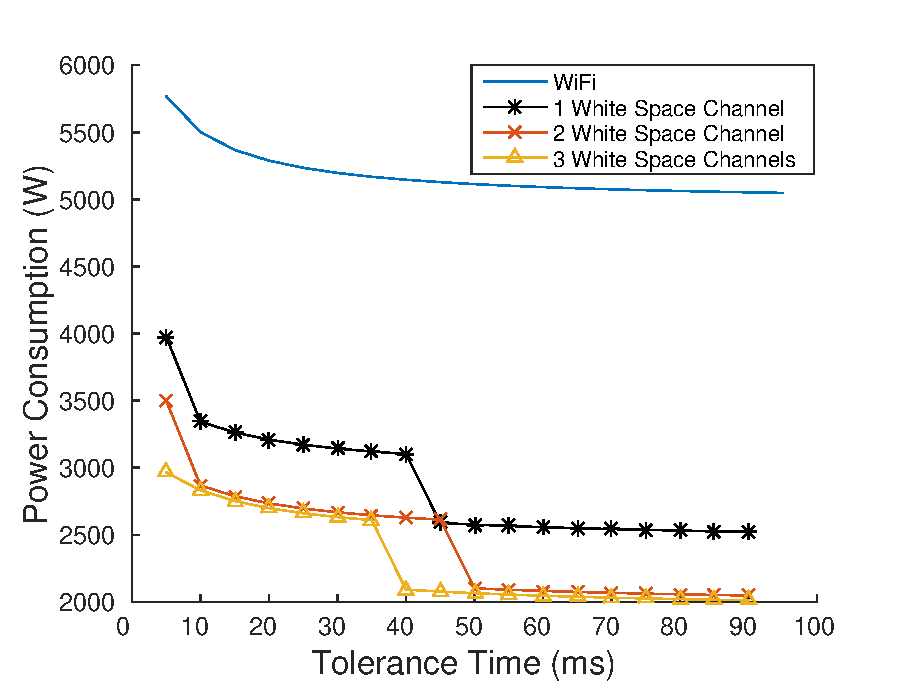
\includegraphics[width=84mm]{figures/delay_vary}
\vspace{-0.1in}
\caption{Power Consumption across Delay Tolerance}
\label{fig:delayvary}
\vspace{-0.1in}
\end{figure}

% Fit for long delay tolerance,if small delay require more resource
From the results shown in Fig.~\ref{fig:delayvary}, we see that the lower the requirement on response time, the less power consumption is required.
As the tolerance response time increase, the power consumption of both WiFi and heterogeneous configuration decreases monotonically. 
The WiFi configuration's power saving mainly stems from the reduction of channel capacity delivery. 
The white space configuration, however, saves power from both the reduction of channel capacity delivery as well as radios turning off. 
With this in mind, we can see sharp reduction in power consumed using the white space configuration in the numerical simulation results due to radios turning off; power consumption shows reduction by 170.24\% with three white space channels under the tolerance response time $90\ ms$.
When the tolerance response time is more than $50\ ms$, there is no great difference between the two white space channels setup and one white space channels setup. 
As discussed in previous section, most of the major cities in the U.S. has restriction of the number of white space channels, thus the network carrier is able to estimate the quality of service they can offer according to the resources available, such as the number of white space channels, the power supply, etc.


Further, we utilize previous measurement work of channel state in multiple cities of DFW metroplex area to study the population density variation in white space network design~\cite{pcuiwinmee}.
For this analysis, we use the achieved channel capacity that maps to the population distribution. 

% Not sentivitv to population? need more resultes
\begin{figure}[hpt]
\vspace{-0.1in}
\centering
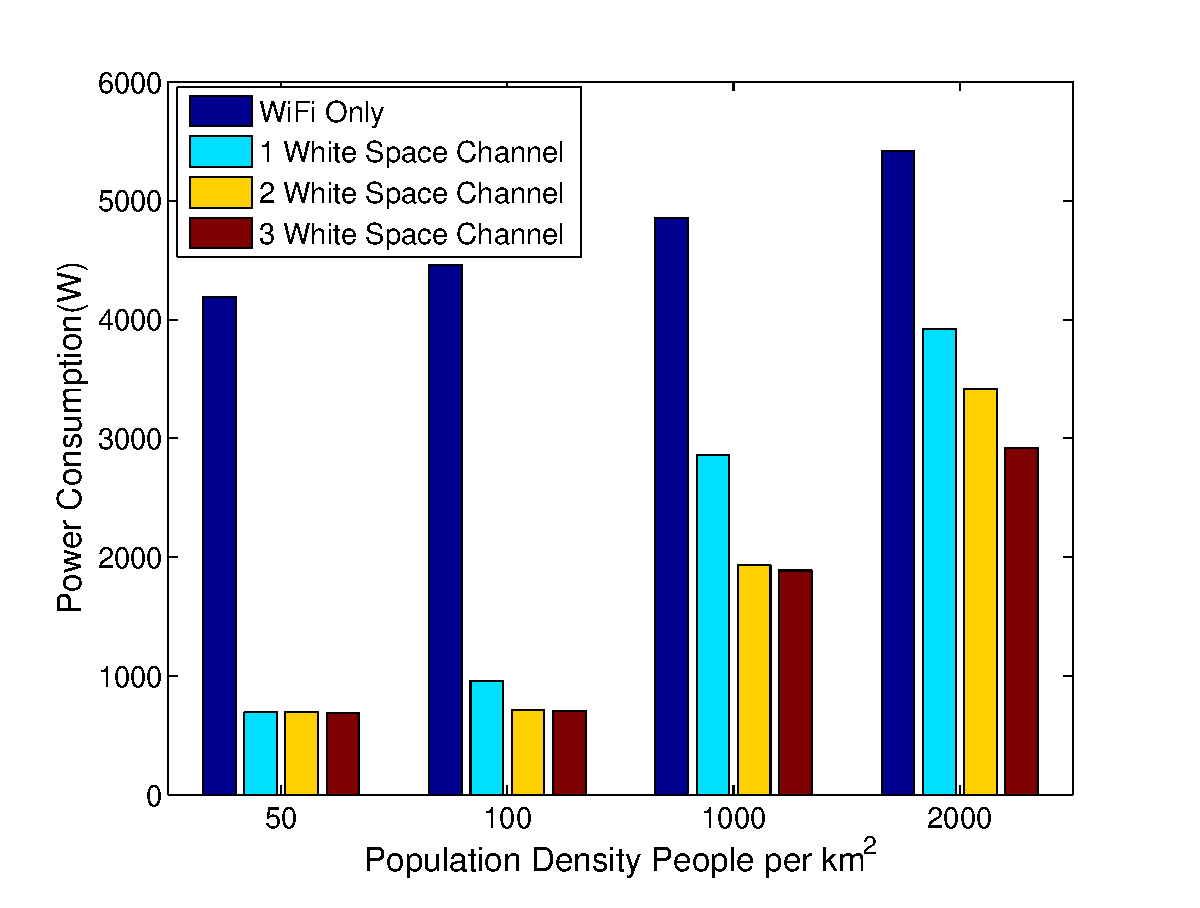
\includegraphics[width=84mm]{figures/populationvary}
\vspace{-0.1in}
\caption{Power Consumption across Population Distribution}
\label{fig:populationvary}
\vspace{-0.1in}
\end{figure}

From the results shown in Fig.~\ref{fig:populationvary}, we see that as the population increases, all the network configurations require more power to serve the users.
The power saving gains of a single white space channel reach their peak, 512.55\%, at a user density of 50 $users/km^2$, and the users are able to be satisfied by only one white space channel. 
Increasing the number of white space channels does not provide any additional reduction in power consumption. 
We see a similar capping out at a user density of 100 $users/km^2$ with two white space channels available; the number of white space channels reaches a point of consistent power consumption increase with the population. 
At a user density of 50 $users/km^2$ this point can be reached using one white space channel while 100 $users/km^2$ needs two white space channels. 
Also, the gain of a single white space channel decrease as the number of white space channels increases.
This diminishing returns effect on the gain can be seen at a user density of 1000 $users/km^2$: the first white space channel gains 70\% of power consumption, the second channel added to the system gains only 47.98\% and the third gains only 2.26\%. 
Therefor, when the number of white space channels are limited, splitting the channels to serve more WiFi cells could decrease power consumption, though the power saved decreases as the population density increase. 




\subsection{Evaluation in Dallas-like Virtual City}
\label{subsec:virtualcity}
In practice, an area that has a stable channel state and constant user mobility does not exist, thus in-field measurements are required to infer the expected performance in the real world.
To evaluate the system performance with a more practical configuration, we query multiple types of areas in Dallas to find the percentage of user activity across time.
In a similar fashion to our prior in-field measurement database query, we pull measurements from downtown areas, urban areas, and suburban neighborhoods around Dallas in areas of fixed size equal to the area of SMU's campus.
Specifically, we use urban area measurements from the eastern of SMU's campus and from North Park mall. 
Suburban neighborhood area measurements were taken from the Highland Park residential area north of campus, from a residential area north of North Park, and from The Village apartment complex east of campus. 
The number of users located in these area are counted according to the GPS locations the distribution of the percentage of users across these areas during a given weekday is recorded in Fig.~\ref{fig:wieyeprocess}. 


\begin{figure}
\vspace{-0.01in}
\centering
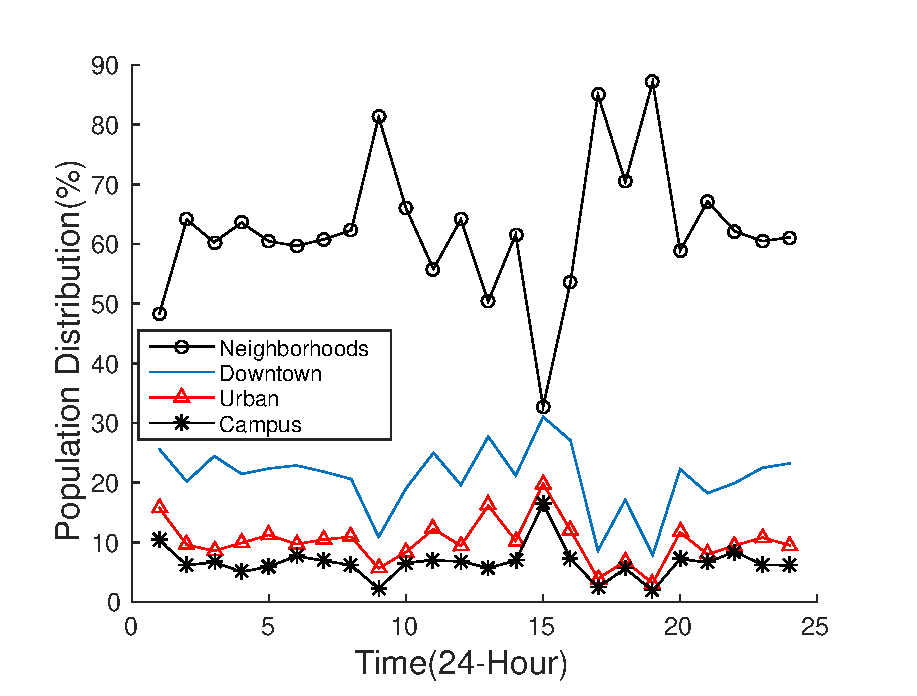
\includegraphics[width=84mm]{figures/wieyeprocess}
\vspace{-0.1in}
\caption{User Distribution across Time}
\label{fig:wieyeprocess}
\vspace{-0.3in}
\end{figure}


The measurements are put in a WhiteCell configuration as previously described, assuming the residents in the city is held constant. 
The channel variation across the spectrum is set up according to both the channel state measurements as well as the user mobility from the measurements results of WiEye discussed in 
Subsection~\ref{subsec:measurements}. The results across 24 hours of the simulated city 
are shown in Fig.~\ref{fig:timevary}

\begin{figure}[hpt]
\vspace{-0.1in}
\centering
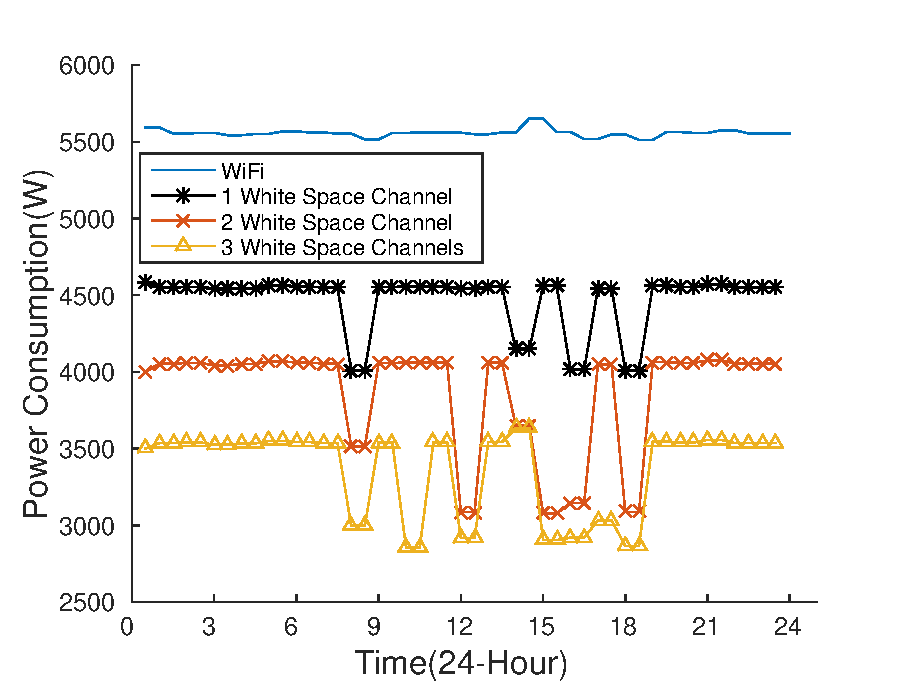
\includegraphics[width=84mm]{figures/timevary}
\vspace{-0.1in}
\caption{Power Consumption across Time}
\label{fig:timevary}
\vspace{-0.1in}
\end{figure}

In this simulation, we observe that the WiFi power consumption remains constant in cases when the users are more uniformly distributed. 
This is because the WiFi radios must be operating in order to serve the users due to the relatively low propagation range. 
The white space radios have the advantage of adapting to the non-uniform user distribution and  mobility. 
When the user distribution changes fast at 9:00 AM, the white space configuration can reduce the power consumed by approximately 20\% compared to the previous user distribution. 
Three white space channels reduce power consumption by nearly half in our results. 
As mentioned earlier, the reduction in power consumption is mainly caused by the ability to turn off the radios when the white space channels are replacing the WiFi channels.
% uniform distribution does not have a great gain
When the users are uniformly distributed, the power consumption may increase due to the division of white space channels. 
The queuing theory concludes that {\it a single, faster server is better than multiple slower servers with the same total capacity}. 
When the users are close to uniformly distributed, the white space channels may be divided into several sub-channels in the algorithm which make the performance worse. 
From the numerical simulation, one white space channel could reduce the power consumed by 24.57\% on average over 24 hours. 
Additionally, our results show that using two white space channels reduces power consumption by 46.27\% and using three white space channels reduces power consumption by 67.40\%. 
Similarly to the previous result, as the number of white space channel increases, the power consumption gains per channel will become constant since there is enough channel capacity to satisfy the users.
According to this result, we can design the network to utilize white space channels, enabling user mobility adaptation and complementing the existing WiFi infrastructure.


% Sum
% WiFi fit for constant user set up
%In the numerical simulation, we leverage the impacts of channel quality, user mobility, quality of service, and population density on the network offloading structure. 
%Further we investigate the performance in a virtual city to simulate the expected in-field performance. 
%Through this simulation, we show that using white space channels can greatly reduce the power consumption of such offloading systems in most scenarios. 
%From our results, we also see the advantage of using white space channels in adapting user mobility to reduce power consumption. 
%Finally, we show how the limited number of white space channels can be a complementary resource for existing WiFi wireless networks, reducing the power consumption and improving the achievable user quality of service. 
